\documentclass[11pt]{article}
\def\nterm {Autumn}
\def\nyear {2022}
\def\nlecturer {A. Chandra, M. Guaraco}
\def\ncourse {Analysis I}
\def\nshort {Analysis I}
\usepackage{amsmath, amsthm, amssymb, amsfonts}
\usepackage{fancyhdr}
\usepackage{xparse, xpatch}
\usepackage[svgnames]{xcolor}
\usepackage[shortlabels]{enumitem}
\usepackage[thinc,text]{esdiff}
\usepackage[bottom]{footmisc}
\usepackage[most]{tcolorbox}
\usepackage{physics}
\usepackage{tikz}
\usepackage{pgfplots}
\usepackage{graphicx, tabularx, caption}
\usepackage{csquotes}
\usepackage[a4paper, left=1.2in, right=1.2in, bottom=1in]{geometry}
\usepackage[hidelinks]{hyperref}
\hypersetup{
    colorlinks,
    allcolors=black
}
\pgfplotsset{compat=1.18}
\graphicspath{{./images/}}

% meta
\setlength{\headheight}{13.6pt}
\renewcommand*\contentsname{Outline}
\pagestyle{fancy}
\lhead{\nouppercase{\leftmark{}}}
\rhead{\nshort}
\title{\textbf{\ncourse}}
\author{Lectured by \nlecturer \\\small Notes taken by Dongshen Wu\footnote{These notes are usually modified significantly after lectures, and are not endorsed by the lecturers at Imperial College, London. They are by no means an accurate representations of what was actually lectured. In particular, all errors are almost surely mine.}}
\date{\nterm \nyear}

% centre tikz pictures
\makeatletter
\g@addto@macro\@floatboxreset\centering
\makeatother

% environment
\tcbset{
  defstyle/.style={
    enhanced, sharp corners,
    attach boxed title to top left={yshift=-2.75mm, 
      xshift=5mm, yshifttext=-2.2mm},
    colback=white, colframe=PeachPuff,
    coltitle=black, fonttitle=\bfseries,
    before skip=7pt,
    boxed title style={sharp corners, size=small,
      colback=PeachPuff,colframe=PeachPuff,}},
  thmstyle/.style={
    enhanced, sharp corners,
    attach boxed title to top left={yshift=-2.75mm, 
      xshift=5mm, yshifttext=-2.2mm},
    colback=AliceBlue, colframe=LightBlue,
    coltitle=black, fonttitle=\bfseries,
    before skip=7pt,
    boxed title style={sharp corners, size=small,
      colback=LightBlue,colframe=LightBlue,}},
  propstyle/.style={
    enhanced, sharp corners,
    attach boxed title to top left={yshift=-2.75mm, 
      xshift=5mm, yshifttext=-2.2mm},
    colback=white, colframe=PowderBlue,
    coltitle=black, fonttitle=\bfseries,
    before skip=7pt,
    boxed title style={sharp corners, size=small,
      colback=PowderBlue,colframe=PowderBlue,}},
}

\newtcbtheorem[number within=section]{TcbThm}{Theorem}{
  thmstyle}{thm}
\NewDocumentEnvironment{theorem}{ O{} O{} }
  {\TcbThm{#1}{#2}}{\endTcbThm}

\newtcbtheorem[number within=section, use counter from=TcbThm]{TcbProp}{Proposition}{
  propstyle}{prop}
\NewDocumentEnvironment{proposition}{ O{} O{} }
  {\TcbProp{#1}{#2}}{\endTcbProp}

\newtcbtheorem[number within=section,use counter from=TcbThm]{TcbDef}{Definition}{
  defstyle}{def}
\NewDocumentEnvironment{definition}{ O{} O{} }
  {\TcbDef{#1}{#2}}{\endTcbDef}

\newtcbtheorem[number within=section,use counter from=TcbThm]{TcbAxi}{Axiom}{
  defstyle}{axi}
\NewDocumentEnvironment{axiom}{ O{} O{} }
  {\TcbAxi{#1}{#2}}{\endTcbAxi}

\newtheorem{corollary}[\tcbcounter]{Corollary}
\tcolorboxenvironment{corollary}{propstyle}
\newtheorem{lemma}[\tcbcounter]{Lemma}
\tcolorboxenvironment{lemma}{propstyle}

\theoremstyle{definition}
\newtheorem*{example}{Example}
\newtheorem*{exercise}{Exercise}
\newtheorem{problem}{Problem}
\newtheorem*{algorithm}{Algorithm}
\newtheorem*{procedure}{Procedure}
\newtheorem*{remark}{Remark}
\tcolorboxenvironment{algorithm}{propstyle}

\theoremstyle{remark}
\newtheorem*{notation}{Notation}
\newtheorem*{solution}{Solution}
\tcolorboxenvironment{solution}{
  blanker,breakable,left=5mm,
  before skip=10pt,after skip=10pt,
  parbox = false,
  borderline west={0.5mm}{0pt}{SlateGray}}
\tcolorboxenvironment{proof}{
  blanker,breakable,left=5mm,
  before skip=10pt,after skip=10pt,
  parbox = false,
  borderline west={0.5mm}{0pt}{SlateGray}}

\newtcolorbox{extension}[1]{
  colback=WhiteSmoke,colframe=Gainsboro, enhanced, before skip=10pt, after skip=10pt, fonttitle=\bfseries,coltitle=black, sharp corners, title={\:\,Extension:\:#1}, before upper app={\setlength{\parindent}{17pt}}
}

% subproof
\makeatletter
\newcounter{subproof}
\xpretocmd{\proof}{\setcounter{subproof}{0}}{}{}
\xpretocmd{\solution}{\setcounter{subproof}{0}}{}{}
\newcommand{\subproof}[1]{%
  \par
  \addvspace{\medskipamount}%
  \stepcounter{subproof}%
  \noindent\emph{Part \thesubproof: #1}\par\nobreak
  \@afterheading
}
\makeatother

% command
\newcommand{\C}{\mathbb{C}}
\newcommand{\N}{\mathbb{N}}
\newcommand{\Q}{\mathbb{Q}}
\newcommand{\R}{\mathbb{R}}
\newcommand{\Z}{\mathbb{Z}}
\renewcommand{\bf}[1]{\mathbf{#1}}
\renewcommand{\cal}[1]{\mathcal{#1}}
\renewcommand{\rm}[1]{\mathrm{#1}}
\newcommand{\floor}[1]{\left \lfloor #1 \right \rfloor}
\newcommand{\ceil}[1]{\left \lceil #1 \right \rceil}
\newcommand{\lointerval}[1]{\ensuremath{\left(#1\right]}}
\newcommand{\rointerval}[1]{\ensuremath{\left[#1\right)}}
% Augmented Matrix
\newenvironment{amatrix}[1]{%
  \left(\begin{array}{@{}*{#1}{c}|c@{}}
}{%
  \end{array}\right)
}

\begin{document}
\maketitle{}
\tableofcontents{}
\pagebreak

%=========================================================
\section{Real numbers}
\subsection{Decimals}
\begin{definition}[Decimals]
  For \(a_0 \in \Z\) and \(a_i \in \{0,1,...,9\}\), we define the decimals \(a_0.a_1a_2...a_i...\) to be 
  \begin{equation*}
    a_0+\frac{a_1}{10}+\frac{a_2}{100}+...+\frac{a_i}{10^i}+...
  \end{equation*}
  for \(a_0 \geq 0\), and for \(a_0<0\), define it to has value \(-(|a_0|.a_1a_2...)\).

  \vspace{5pt}It is finite if exists \(j\) such that \(a_i=0\) for all \(i \geq j\).

  \vspace{5pt}It is eventually periodic if for some \(i,j\), the decimal is
  \begin{equation*}
    a_0+\frac{a_1}{10}+\frac{a_2}{100}+...+\frac{a_i}{10^i}+\frac{a_{i+1}a_{i+2}...a_j}{10^j(1-10^{i-j})}
  \end{equation*}
  denoted as \(a_0.a_1a_2...a_i\overline{a_{i+1}a_{i+2}...a_j}\). Note the numerator in the last fraction is a string of numbers not a product.
\end{definition}

The definition of eventually periodic number is motivated by the `infinite geometric sum result' (which is yet to be proved).
\begin{exercise}
  Consider two eventually periodic decimals \(a,b\) differing at the nth index only i.e. \(a_n \neq b_n\) for exactly one \(n\). Show that \(a<b\) if and only if \(a_n<b_n\).
\end{exercise}
\begin{solution}
  This is quite trivial from the definition.
\end{solution}

\begin{theorem}
  Any \(x \in \Q\) is equal to an eventually periodic decimals.
\end{theorem}
\begin{proof}
  Wlog, let \(x\geq 0\). To write \(x\) as decimal, we let \(a_0:=\floor{x}\) and \(e_0:=\{x\}\), the integer and fractional part respectively. Hence \(x=a_0+e_0\).
  We then repeat for \(10e_0\), with \(a_1:=\floor{10e_0}\) and \(e_1:=\{10e_0\}\).
  Inductively, we have \(10e_{k-1}=a_k+e_k\) for \(k\geq 1\).
  Put each equation into the former gives, for arbitrary \(k\), 
  \[x=a_0+\frac{a_1}{10}+...+\frac{a_k}{10^k}+\frac{e_k}{10^k}\]
  
  Define \(qe_k:=r_k\) for \(k\in\N\). Recall that \(x=\frac{p}{q}\) is rational, so \(p=qa_0+qe_0=qa_0+r_0\) is an integer. In particular, \(r_0 \in \{0,1,...q-1\}\) is the remainder of \(p\) modulo \(q\). Inductively, \(q10e_{k-1}=q(a_k+e_k)=qa_k+r_k\) is also an integer, so \(r_k \in \{0,1,...,q-1\}\) also. Since \(\{0,1,...,q-1\}\) is finite, we must have some \(i<j\) such that \(r_i=r_j\) and thus \(e_i=e_j\).

  \vspace{5pt}In order to show \(x=a_0.a_1...a_i\overline{a_{i+1}a_{i+2}...a_j}\), all we need to show now is 
  \begin{align*}
    \frac{e_i}{10^i} &= \frac{a_{i+1}a_{i+2}...a_j}{10^j(1-10^{i-j})} & \text{or equivalently,} & &(10^{-i}-10^{-j})e_i=\frac{a_{i+1}a_{i=2}...a_j}{10^j}
  \end{align*}

  But using \(e_i=e_j\) and \(a_k=10e_{k-1}-e_k\), we have
  \begin{align*}
    (10^{-i}-10^{-j})e_i&=\frac{e_i}{10^i}-\frac{e_j}{10^j}\\
    &=(\frac{e_i}{10^i}-\frac{e_{i+1}}{10^{i+1}})+(\frac{e_{i+1}}{10^{i+1}}-\frac{e_{i+2}}{10^{i+2}})+...+(\frac{e_{j-1}}{10^{j-1}}-\frac{e_j}{10^j})\\
    &=\frac{a_{i+1}}{10^{i+1}}+\frac{a_{i+2}}{10^{i+2}}+...+\frac{a_j}{10^j} 
    = \frac{a_{i+1}a_{i+2}...a_j}{10^j}
  \end{align*}
\end{proof}

Some different eventually periodic decimals would give the same rational number.

\begin{example}
  Show that \(0.\bar{9}=1\).
\end{example}
\begin{solution}
  By definition, \(0.\bar{9}=\frac{9}{10(1-10^{-1})}=1\).\qed
\end{solution}

Turns out this is the only case we need to worry about.
\begin{proposition}
  If \(x\in\Q\) has two different decimal expansions, then they are of the form
  \[x=a_0.a_1...a_n\bar{9}=a_0.a_1...(a_n+1)\]
  where \(a_n\in\{0,1,...,8\}\).
\end{proposition}
\begin{proof}
  Suppose wlog that \(x=a_0.a_1...a_na_{n+1}...=a_0.a_1...b_nb_{n+1}...\) where \(a_n<b_n\).
  Then by previous exercise,
  \begin{align*}
    x &= a_0.a_1...a_na_{n+1}... \\
      &\leq a_0.a_1...a_n999... \\
      &= a_0.a_1...(a_n+1)000... \\
      &\leq a_0.a_1...b_nb_{n+1}... = x
  \end{align*}
  Thus the inequalities must be equality, so we are done.
\end{proof}

This allow us to define the real numbers uniquely.
\begin{definition}[Real numbers]
  The reals \(\R\) is the set of arbitrary decimals which does not end in \(\bar{9}\).
\end{definition}

\subsection{Countability}
\begin{definition}[Countably infinite]
  A set \(S\) is countably infinite if there exists a bijection \(f:\N \to S\) (or equivalently a bijection \(g:S \to \N\) due to existence of two-sided inverse.)

  \vspace{5pt}A set is said to be countable if it is finite or countably infinite, otherwise it is uncountable.
\end{definition}
Clearly, \(\N\) is countable. The identity map would do the job.

\begin{proposition}[Subset of \(\N\) is countable][CountableSubset]
  Any \(S \subset \N\) is countable.
\end{proposition}
\begin{proof}
  If \(S\) is finite, then we are done.

  Otherwise, we list the elements of \(S\) in order of size as it is well-ordered. We defined \(f:\N \to S\) inductively as:
  \begin{itemize}
    \item \(f(1):=\min(S)\)
    \item \(f(n):=\min(S\backslash\{f(1),f(2),...,f(n-1)\})\). The set is non-empty as \(S\) is infinite.
  \end{itemize}
  Essentially just assign an increasing order to \(S\). We just need to show \(f\) is a bijection.

  The function is clearly injective since \(f(1)<f(2)<...\). Suppose \(f\) is not surjective, then there exists a smallest \(s\) that is not in the image of \(f\). Since \(s\neq \min(S)\) by definition, we know there exist \(s'\in S\) such that \(s'<s\). Pick the largest such \(s'=f(n)\), then by definition \(s=f(n+1) \in S\), a contradiction.
\end{proof}

\begin{proposition}[][CountFunc]
  \begin{enumerate}
    \item If there exists an injection \(f:A\to B\) and \(B\) is countable, then \(A\) is countable.
    \item If there exists a surjection \(f:A\to B\) and \(B\) is uncountable, then \(A\) is uncountable.
  \end{enumerate}
\end{proposition}
\begin{proof}
  \subproof{}
  Let \(f(A)\) be the image of \(A\). Then \(f:A\to f(A)\) is a bijection. Since \(f(A)\) is a subset of \(B\), \(f(A)\) is countable, meaning there exists bijection \(g:f(A)\to \N\). It follows that \(g\circ f:A\to \N\) is a bijection, so \(A\) is countable.
  \subproof{}
  Let %TODO
\end{proof}

\begin{theorem}[\(\Q\) is countable][CountableQ]
  The set of rational numbers \(\Q\) is countably infinite.
\end{theorem}
\begin{proof}
  First, lets show that \(\Q_>:=\{x\in\Q:x>0\}\) is countably infinite. We define an injection \(f:\Q_> \to \N\) as
  \begin{equation*}
    f(m/n):=2^m3^n
  \end{equation*}
  where \((m,n)=1\). Clearly \(f\) is injective, so \(\Q_>\) is countable by proposition \ref{prop:CountFunc}, i.e. has bijection \(F:\Q_>\to\N\).

  Now, we define a bijection \(g:\N \to \Q\) in a similar fashion to the proof of \(\Z\):
  \[\text{For } k\in \N,\begin{cases}
    g(0)&=0 \\
    g(2k)&=F(k)\\
    g(2k+1)&=-F(k)
  \end{cases}\]
  This is clearly injective and surjective (as \(\Q = \Q_<\cup\{0\}\cup\Q_>\)).
\end{proof}

\begin{corollary}
  \label{CountableCarte}
  Any \emph{finite} Cartesian product of countable sets is countable.
\end{corollary}
\begin{proof}
  Firstly, any countable set has a bijection with \(\N\), so it is sufficient to show that \(\N^k\) is countable for all \(k\in\N\).

  The proof of this follows the same process as the first part of proof of theorem \ref{thm:CountableQ}. For \(k\in\N\) times Cartesian product, we define f: \(\N^k \to \N\) as 
  \begin{equation*}
    f((x_1,...,x_k)):=p_1^{x_1}...p_k^{x_k}
  \end{equation*}
  where \(p_i\) are distinct primes. Since there are countably infinitely many primes, this works for any \(k \in \N\). This is clearly injective, so by proposition \ref{prop:CountFunc} we are done. 
\end{proof}
\begin{remark}
  Note that the if \(k\) becomes \emph{countably infinite}, then the Cartesian product essentially becomes a countably infinite string of arbitrary numbers, which is \emph{not} countable by using Cantor's diagonal argument for the reals as described later.
\end{remark}

\begin{proposition}[Countable union of countable sets is countable][CountableUnion]
  If \(S_i\) is countable for all \(i\in\N\), then \(A:= \bigcup_{i\in\N}S_i\) is also countable.
\end{proposition}
\begin{proof}
  By definition, there exists bijection \(f_i:S_i\to\N\) for all \(i\in\N\). Then define \(f:A\to\N^2\) as: if \(x \in S_i\), then \(x \mapsto (i,f_i(x))\), pick an arbitrary one if is in multiple \(S_i\). This is clearly injective. By proposition \ref{prop:CountFunc}, \(A\) is countable.
\end{proof}

\begin{problem}
  Prove that \(\Omega = \{S\subset\N:|S| \in \N\}\), the set of finite subsets of \(\N\), is countable.
\end{problem}
\begin{solution}
  Define \(\Omega_n := \{S\in\Omega:|s|=n\}\) for \(n\in\N\), so \(\Omega=\bigcup_{i\in\N}\Omega_i\). By lemma \ref{prop:CountableUnion}, all we need to show is \(\Omega_i\) is countable \(\forall i\). 

  \vspace{5pt}Consider arbitrary \(k\in\N\). Define \(f_k:\Omega_k\to\N^k\) as the function that take \(S\in\Omega_k\) to \((s_1,s_2,...,s_k)\) where \(s_i\) are elements of \(S\) and \(s_1<s_2<...<s_k\). It is clear that \(f_k\) is injective. Then, by lemma \ref{CountableCarte}, there exists bijection \(g:\N^k\to\N\). Hence \(h_k=g\circ f_k\) is injection, i.e. \(\Omega_k\) is countable by proposition \ref{prop:CountFunc}.\qed

  \vspace{5pt}Alternatively, we can define a function \(f:\Omega\to\Q\) by using counting ideas, namely, for \(S \in \Omega\),
  \[f(S)=0.b_0b_1...b_n... \text{ where } b_i=\begin{cases}
    1 & \text{if } i \in S \\
    0 & \text{if } i \notin S \\
  \end{cases}\]
  We essentially assign an unique binary string for each \(S\) and convert it into decimal. Since \(S\) is finite, we must have some \(i\) where \(b_j=0\) for all \(j>i\), so \(f(S)\) is finite decimals. Hence \(f(S)\subset \Q\), which is countable.
  \qed
\end{solution}

\begin{proposition}[\(\mathcal{P}(\N)\) is uncountable]
  The power set (set of subsets) of \(\N\) is uncountable.
\end{proposition}
\begin{proof}
  Suppose we have a countable list of all subsets of \(\N\): \[S^1=\{s_1^1,s_2^1,...\},S^2=\{s_1^2,s_2^2,...\},...,S^n=\{s_1^n,s_2^n,...\},...\] Since they are well-ordered, we define them so that \(s_i^n<s_{i+1}^n\) for all \(i,n\).

  \vspace{5pt}We define \(t_n\in\N\) recursively by \(t_n=\max(s_n^n,t_{n-1})+1\). We want to show that \(T = \{t_1,t_2,...\} \subseteq \N\) is not equal to any of \(S^i\), and thus a new set outside of the exhaustive list, a contradiction. In a sense, it is similar to Cantor's diagonal argument.

  \vspace{5pt}To do this, let's suppose \(T=S^n\) for some \(n\in\N\). Since both sequence in \(S^n\) and \(T\) are increasing by definition, they can only be equal if and only if \(t_i=s_i^n\) for all \(i\). 

  \vspace{5pt}Consider \(i=n\). If \(s_n^n>t_{n-1}\), then \(t_n=s_n^n+1=s_n^n\), a contradiction. If \(t_{n-1}>s_n^n\), then \(t_n =t_{n-1}+1=s_n^n\), but that means \(t_{n-1}<s_n^n\), again a contradiction.
\end{proof}

\begin{theorem}[\(\R\) is uncountable]
  The set of real numbers \(\R\) is uncountable.
\end{theorem}
\begin{proof}
  We finally introduce the \emph{Cantor's diagonal argument}. Suppose all real numbers can be listed using \(\N\) as index set, i.e. we have all reals in a list of \(x_i\) where 
  \[x_{i}=a_{i}.a_{i1}...a_{ij}...\text{ such that } i \in \N; a_i \in \Z; a_{ij} \in \{0,1,...,9\}, \forall i,j\]

  Now we produce a number that is not on the list:
  \[x:=0.b_1b_2...b_n... \text{ such that } b_n \in \{0,1,...,8\} \text{ and } b_n \neq a_{nn}, \forall n\]

  Since we don't include 9, we cannot end up with \(\bar{9}\). Then we see \(\forall i, x \neq x_i\) as they differ in the \(i\)th decimal place.,
\end{proof}

\begin{exercise}
  Let \(A\) be uncountable and \(B\subset A\) be countable. Is \(A\backslash B\) always uncountable?
\end{exercise}
\begin{solution}
  Suppose \(A\backslash B\) is countable. Since \(B\) is countable, so by lemma \ref{prop:CountableUnion}, \((A\backslash B)\cup B\) is countable. But clearly \(A\subseteq (A\backslash B)\cup B\), that is, \(A\) is contained in a countable set so must be a countable set itself, a contradiction.\qed 
\end{solution}

\begin{extension}{Continuum hypothesis}
  As a member of the millenium problems proposed by Hilbert, the Continuum hypothesis states that: there is no set whose cardinality is strictly between that of the integers and the real numbers (the countable and the uncountable). In ZFC, this can be denoted using \emph{aleph numbers}:
  \begin{equation*}
    2^{\aleph_0}=\aleph_1
  \end{equation*}

  This hypothesis has been proven to be logically independent from ZFC (i.e. cannot be proved or disproved from it) by Kurt Gödel and Paul Cohen.
\end{extension}

\begin{problem}
  Let \(A\) be the set of all function \(f:\N\to\N\). Is the following sets countable:
  \begin{enumerate}
    \item \(\{f\in A: \exists n\in\N, \forall a\in\N, f(a+n)=f(a)\}\) (the set of periodic function)
    \item \(\{f\in A: f(a)=f(b) \implies a=b\}\) (the set of injective function)
    \item \(\{f\in A: \forall \epsilon >0, \exists N\in\N, \forall n\geq N, |f(n)|<\epsilon\}\) (the set of function with limit 0)
  \end{enumerate}
\end{problem}
\begin{solution}
  %TODO
\end{solution}

\begin{definition}[Algebraic number]
  The set of algebraic number is defined as \(\mathbb{A}:=\{x\in\R:p(x)=0\}\) where \(p\) is a polynomial with integer coefficients, \(\Q \subset \mathbb{A} \subset \R\).
  
  \vspace{5pt}Real numbers that are not algebraic are called \emph{transcendental}.
\end{definition}

\begin{proposition}[Countability of algebraic number]
  The set of algebraic number is countable while the set of transcendental is not.
\end{proposition}
\begin{proof}
  First note that the set of polynomial with integer coefficients is countable. This is because a polynomial of degree \(k-1\) can be thought as a list of \(k\) integers representing the coefficients, i.e. in the space \(\Z^k\), which is countable by corollary \ref{CountableCarte}.
  
  Since each polynomial has a finite number of roots, we may replace each polynomial with their roots in the list and still obtain a countable list. This contains all algebraic number (with repetition even). Hence \(\mathbb{A}\) is countable.

  Since \(\R\) is uncountable, \(\R\backslash\mathbb{A}\), the set of transcendental numbers, must be uncountable, by previous exercise.
\end{proof}

% \begin{problem}
%   Prove that every root of a monic polynomial (leading coefficient is 1) with integer coefficients is either irrational or integer.
% \end{problem}

%----------------------------------------------------
\subsection{Ordered set}
Recall the definition of bound from ``Introduction to Univeristy Mathematics'', and that \(\R\) needs to satisfy the completeness axiom. This is what we would show in this section. We would also present an alternative construction of the reals.

\begin{definition}[Ordered set]
  An ordered set \(S\) is a set with with an order, \(<\), satisfying
  \begin{enumerate}
    \item (Trichotemy) If \(x,y\in S\), then exactly one of \(x<y,x=y,y<x\) is true.
    \item (Transitive) If \((x,y,z)\in S\) and \(x<y,y<z\), then \(x<z\)
  \end{enumerate}
\end{definition}

\begin{definition}[Upper bound and supremum]
  For an ordered set \(S\) and a non-empty subset \(X\subset S\), \(a\) is an upper bound of \(S\) if \(a\geq x\) for all \(x\in X\). 

  It is a least upper bound, or supremum, if \(b\) is not an upper bound for any \(b<a\).

  Lower bound and infimum is defined similarly.
\end{definition}

Here is a rather useful proposition when proving things about supremum.
\begin{proposition}[][1]
  Suppose \(S\subset \R\) is non-empty and bounded above by \(y\). Then \(y=\sup S \iff \forall \epsilon>0, \exists s\in S \text{ such that } s>y-\epsilon\).
\end{proposition}
\begin{proof}
  \subproof{\(\implies\)}
  By definition, \(y-\epsilon\) is not upper bound for \(\epsilon >0\), so exists \(s\in S\) such that \(s>y-\epsilon\).
  \subproof{\(\impliedby\)}
  Suppose \(x<y\) and \(x\) is an upper bound. Set \(\epsilon=y-x>0\) gives \(s>x\), a contradiction.
\end{proof}

\begin{exercise}
  Take bounded, non-empty \(S,T\subset\R\), define \(S+T:=\{s+t:s\in S,t\in T\}\). Show that
  \[\sup(S+T)=\sup(S)+\sup(T)\]
\end{exercise}
\begin{proof}
  By definition, \(s\leq \sup(S)\) and \(t\leq \sup(T)\) for all \(s,t\) so \(\sup(S+T)\leq \sup(S)+\sup(T)\). By proposition \ref{prop:1}, for all \(\epsilon>0\), exists \(s>\sup(S)-\epsilon \in S\) and \(t>\sup(T)-\epsilon\in T\). Hence exists \(s+t > \sup(S)+\sup(T)-2\epsilon\). Thus
  \[\sup(S)+\sup(T)-2\epsilon<\sup(S+T)\leq\sup(S)+\sup(T)\]
  which implies \(\sup(S+T)=\sup(S)+\sup(T)\) by taking the limit \(\epsilon\to 0\).
\end{proof}


\begin{definition}[Least upper bound property]
  An ordered set \(S\) is said to have the least upper bound property if for all \(A\subset S\) non-empty and bounded above, \(\sup A\in S\).
\end{definition}
This is a form of the completeness axiom. Some other common equivalent forms are Dedekind completeness, Cauchy completeness, and Bolzano-Weierstrass theorem, which we would discuss later.

It turns out that every ordered set with the least upper bound property also has the greatest lower bound property.
\begin{theorem}[Equivalence to greatest lower bound property]
  Suppose \(S\) is an ordered set with the least upper bound property, and \(B \subset S\) is non-empty and bounded below. Let \(A\) be the set of all lower bounds of \(B\), Then \[\exists \alpha \in S \text{ such that } \alpha = \sup A = \inf B\] 
\end{theorem}
\begin{proof}
  Since \(B\) has lower bound, \(A\) is not empty. Since \(A\) consists of exactly those \(y\in S\) satisfying \(y\leq x\) for all \(x\in B\), we see that every \(x\in B\) is an upper bound of \(A\), so \(A\) is bounded above. By the least upper bound property, \(\alpha:=\sup A\) exists in \(S\).

  If \(\gamma<\alpha\), then by definition \(\gamma\) is not an upper bound of \(A\), so \(\gamma \notin B\). Hence \(\alpha \leq x\) for all \(x\in B\). Thus \(\alpha \in A\).

  If \(\alpha < \beta\), then \(\beta \notin A\), since \(\alpha\) is an upper bound of \(A\).

  We have thus shown that \(\alpha \in A\) but \(\beta \notin A\) if \(\beta > \alpha\). That is, \(\alpha\) is a lower bound of \(B\), but \(\beta\) is not if \(\beta > \alpha\). This by definition means that \(\alpha = \inf B\).
\end{proof}

\begin{theorem}[Least upper bound property of arbitrary decimals]
  The set of arbitrary decimals satisfies the least upper bound property, that is,if \(S \subset \R\) is non-empty and bounded above, then \(S\) has a supremum in \(\R\).
\end{theorem}
\begin{proof}
  \subproof{Simplify the problem}
  WLOG, we may assume \(S\neq\emptyset\) has a positive element \(0\leq s\in S\), as we can always translate \(S\) by a big enough number.

  Then, since \(S\) is bounded above, say, by \(N\in\N\), we can equivalently consider the supremum of \(S\cap [0,N]\) (exercise). Thus we don't need to worry about negative decimals.

  \subproof{Build a candidate for supremum}
  For the rest of the argument, we refer to \(a=a_0.a_1a_2...\) as our supremum and \(s=s_0.s_1s_2...\) an arbitrary element in \(S\).

  Since \(s\in [0,N]\), we see \(s_0\in\{0,1,...,N\}\), a finite set, so we have a maximum \(s_0\) in this set, call it \(a_0\).

  Then, \(S\cap \rointerval{a_0,a_0+1}\) is non-empty, so replace \(S\cap [0,N]\) with this just like we did at the start. Now, \(s_1\in\{0,1,...,9\}\), a finite set, so we have a maximum \(s_1\) in this set, call it \(a_1\).

  It is then clear that this argument continues inductively, where we consider the set \(S\cap \rointerval{a_0.a_1...a_{n-1},a_0.a_1...(a_{n-1}+1)}\) for the \(n\)th decimal place.

  \subproof{Prove \(a\) is the supremum}
  It is clear by our construction that \(s_i \leq a_i\) for all \(i\), so \(a\) is an upper bound. We now need to show that it is the least such bound.

  Suppose \(b<x\) and \(b\) is an upper bound for \(S\). Suppose also that they differ from \(a\) in the \(n\)th digit. In particular, \(b=a_0.a_1...a_{n-1}b_n...\) where \(b_n<a_n\).

  But there exists element in \(S\) with \(a_0.a_0...a_{n-1}a_n...\) by construction, and so \(s>b\), i.e. \(b\) is not an upper bound.
\end{proof}

\begin{exercise}
  Show that there exists \(x \in \R\) such that \(x^2=3\).
\end{exercise}
\begin{solution}
  Set \(S=\{a\in\R:a^2<3\}\). Clearly \(S\) is non-empty as \(1\in S\). Hence by completeness theorem, there exists \(x:=\sup S\). Want to show that \(x^2=3\). We can do this by showing \(x^2\) is not smaller or not bigger than \(3\).
  Also, 2 is clearly an upper bound. 

  Suppose \(x^2<3\). Consider \((x+\epsilon)^2 = x^2+2\epsilon x+ \epsilon^2 < x^2+(2x+1)\epsilon \leq x^2+5\epsilon<3\) if \(\epsilon\leq 1\)so set, say, \(\epsilon_0=\min(1,\frac{3-x^2}{10})\). Then any \(y\in (x,x+\epsilon_0)\) satisfies \(y^2<3\) so \(y\in S\) but \(y>x\), so \(x\) is not an upper bound, a contradiction.

  Similarly, suppose \(x^2>3\). Consider\((x-\epsilon)^2 \geq x^2-2\epsilon \geq x^2 - 4\epsilon>3\), so set \(\epsilon_0 = \frac{x^2-3}{4}\). If \(y \in (x-\epsilon_0, x)\), then \(y^2>3\) is an upper bound of \(S\), but \(y<x\), so x is not the least upper bound, a contradiction.

  Thus by trichotemy, \(x^2=3\) exists in \(\R\).
\end{solution}

\subsection{Dedekind cut}

Now, let's present an alternative way to construct the reals from the rationals. Intuition: \(S_r = (-\infty,r)\cap\Q\), then \(r_1=r_2 \iff S_{r_1}=S_{r_2}\).
\begin{definition}[Dedekind cut]
  A Dedekind cut is any set \(a\subset\Q\) satisfying  
  \begin{enumerate}[label={(\Roman*)}]
    \item \(a\neq\emptyset, a\neq\Q\)
    \item If \(x\in\Q,y\in a,\text{ and } x<y \), then \(x\in a\).
    \item If \(x\in a\), then exists \(y\in a\) such that \(y>x\).
  \end{enumerate}
  So essentially, a proper subset \(a\in\Q\) is a Dedekind cut if it closed downwards and does not contain a greatest element.
\end{definition}
Here I use a lowercase instead of an uppercase to indicate the one-to-one relation of a cut with a real number, as we will see later. We would obtain the extended real number line formally if we ignore the requirement of \(a\) being \emph{proper} subset (so \(-\infty=\emptyset,\:\infty=\Q\)).

\begin{theorem}[Dedekind completeness of \(\R\)]
  There exists an ordered field \(\R\) that has the least upper bound property, and contains \(\Q\) as a subfield.

  In fact, \(\R\) can be constructed as the set of all Dedekind cuts \(S\subset\Q\).
\end{theorem}
\begin{proof}
  There are 2 implications from the 2nd condition of cut that we would use freely throughout the proof: \[p\in S \land q\notin S \implies p<q; \:\:p\notin S \land p<q \implies q \notin S\]
  \subproof{Ordered set}
  We define an order on \(\R\) as \(a<b\) if \(a\) is a proper subset of \(b\). It is clear that \(<\) is transitive, and at most one of the \(a<b,a=b,b<a\) holds. To show at least one holds, we assume WLOG the first two fails. Then since \(a\) is not a subset of \(b\), exists \(p\in a\) such that \(p\notin b\), so if \(q\in b, q<p\), i.e. \(q\in a\). Thus \(b\subset a\). Since \(a\neq b\), we have \(b<a\).

  Hence \(\R\) is an ordered set.
  \subproof{Least upper bound property}
  Let \(A\subset\R\) be non-empty, and assume that \(b \in\R\) is an upper bound of \(A\). Let \(c\) be the union of cuts \(a\) in \(A\). We shall prove that \(c\in\R\) and \(c=\sup A\).

  Since \(A\) is non-empty, exists \(a_0\in A\), which is non-empty. Since \(a_0\in c\), \(c\neq\emptyset\). Since \(a<b \: \forall a\in A\), we have \(c<b\), so \(c\neq\Q\). This proves (I). Next, pick some \(p\in c\), say, \(p\in a_1\in A\). If \(q<p\), then \(q\in a_1\) i.e. \(q\in c\). This proves (II). If another \(r\in a_1\) is chosen that \(r>p\) (we can do that as \(a_1\in\R\)), then \(r\in c\) since \(a_1<c\). This proves (III). Hence \(c\in\R\).

  It is clear by our defintion that \(a<c\) or \(a=c\) for all \(a\in A\), so \(c\) is an upper bound. Suppose \(d<c\), then exists \(s\) such that \(s\in c\) and \(s\notin d\). Then, since \(s\in c\), \(s\in a_2\) for some \(a_2\in A\), so \(d <a_2\). Hence \(d\) is not an upper bound. Thus \(c=\sup A\).
  \subproof{Addition axiom}
  We define addition on \(\R\) as \(a+b:=\{r+s:r\in a\land s \in b\}\). We define \(0^*\) the rational cut as the set \(\{s\in\Q:s<0\}\), and use this in place of \(0\). We would show that \(a+b\) is a cut, and furthermore (A1-4) holds for this definition.

  (A1):%TODO Rudin
  \subproof{Ordered field}
  \subproof{Multiplication axiom}
  \subproof{\(\Q\) is a subfield of \(\R\)}
\end{proof}

\begin{theorem}[Triangle inequality (main)]
  For all \(a,b \in\R\) we have \[|a+b|\leq |a|+|b|\]
\end{theorem}
\begin{proof}
  Suppose \(|a+b|>|a|+|b|\). Then \((|a+b|)^2>(|a|+|b|)^2\) or \(a^2+2ab+b^2>|a|^2+2|a||b|+|b|^2\). But \(ab\leq |a||b|\) so in fact the opposite inequality hold. 
\end{proof}

\begin{proposition}
  \(\forall \epsilon >0, |x-a|<\epsilon \iff x=a\)
\end{proposition}
\begin{proof}
  Suppose \(x\neq a\). Then \(|x-a|>0\). Let \(\epsilon=\frac{1}{2}|x-a|>0\). But \(|x-a|<\frac{1}{2}|x-a| \implies \frac{1}{2}|x-a|<0 \implies |x-a|<0\), contradiction.
\end{proof}

%=========================================================
\section{Sequences}
\subsection{Limit and convergence}
\begin{definition}[Sequence]
  A sequence \((a_n)\) is a function \(a:\N \to \R\) where we let \(a_n\in\R\) denote \(a(n)\) for \(n\in\N\).
\end{definition}


There are a few ways to characterise a sequence: list, closed formula, recursion, series.

\begin{exercise}
  Show any sequence \((a_n)\) is a sequence of partial sums of another sequence, i.e. can be written as a series \(a_n=\sum_{i=1}^nb_i\).
\end{exercise}

We want to rigorously define the concept of limit, i.e. \(a\) is the limit of \((a_n)\). Here is the idea: \(a_n\) should be able to get as close to \(a\) as we want by going sufficiently far down the sequence. Formally,
\begin{definition}[Limit of sequence]
  We say that \(a_n\to a\) as \(n\to\infty\) if and only if for all \(\epsilon >0\) (fixed), there exists \(N\in\N\) such that for all \(n\geq N\), \(|a_n-a|<\epsilon\). In symbols, this is
  \[\forall \epsilon >0, \exists n\in\N \text{ such that } \forall n\geq N, |a_n-a|<\epsilon\]
\end{definition}

\begin{exercise}
  Prove \(1/n \to 0\) as \(n\to\infty\).
\end{exercise}
\begin{solution}
  Let \(\epsilon >0\). Let \(N_\epsilon=\ceil{1/\epsilon}+1\). Then for \(n\geq N_\epsilon\), we have \(|1/n-0|=1/n\leq 1/N_\epsilon < \epsilon\). (We work backwards but write our proof forward.)
\end{solution}

A common way to prove \(a_n\to a\) is: Fix \(\epsilon>0\). Calculate \(|a_n-a|\) and find a good estimate \(|a_n-a|\leq b_n\). Try to solve \(b_n\leq\epsilon\). Find \(N_\epsilon\in\N\) such that above holds for all \(n\geq N_\epsilon\). Finally, write proof logically (usually in reverse order).

\begin{example}
  Prove \(a_n=\frac{n+2}{|n-2|\to 1}\).

  \emph{Rough work:} 
  We can drop the absolute value as we can always make \(N_\epsilon>2\) e.g. using \(\max\). Then \(|a_n-1|=\frac{4}{n-2}\). Want to find \(N_\epsilon\) such that \(n>N_\epsilon\implies\frac{4}{n-2}<\epsilon\). So we need a bigger and more managable estimate for the fraction. To do this, we can make \(2\) in the denominator bigger. For example, \(2<\frac{n}{2}\) for \(n>4\), then \(\frac{4}{n-2}<\frac{4}{n-n/2}=\frac{8}{n}<\epsilon\) if \(n>\frac{8}{\epsilon}\) also. Hence set \(N_\epsilon=\max\{4,\frac{8}{\epsilon}\}\).

  \vspace{5pt}\emph{Written proof:}
  For an arbitrary \(\epsilon\), by setting \(N_\epsilon=\max\{4,\frac{8}{\epsilon}\}\), we have for all \(n>N_\epsilon\) (i.e. \(n>\frac{8}{\epsilon}\) \emph{and} \(n>4\)),
  \[\left|\frac{n+2}{|n-2|}-1\right|=\frac{4}{n-2}<\frac{4}{n-n/2}=\frac{8}{n}<\epsilon\]
\end{example}

It makes intuitive sense that we don't have to get exactly \(\epsilon\) on the right hand side to show convergence. Any independent scalar should work as long as the right hand side can be made arbitrarily small.
\begin{proposition}
  For any constant \(c>0\) (independent on \(\epsilon,n,N\)), \(a_n\to a\) if and only if 
  \[\forall \epsilon >0, \exists n\in\N \text{ such that } \forall n>\N, |a_n-a|<c\epsilon\]
\end{proposition}
\begin{proof}
  Apply definition to \(\epsilon'=c\epsilon\) and \(\epsilon'=\epsilon/c\) for each direction respectively.
\end{proof}

\begin{definition}[Convergence]
  A sequence is convergent if and only if it has a limit. Otherwise it is divergent.
\end{definition}

\begin{exercise}
  We usually define the limit of complex sequence by replacing the aboslute value with \(|z|=\sqrt{(\Re z)^2+(\Im z)^2}\) in the definition of real limits. Show that this condition for complex convergence is equivalent to \(\Re a_n\to\Re a\) and \(\Im a_n\to\Im a\).
\end{exercise}

\begin{theorem}[Limits are unique]
  If \(a_n\to a\) and \(a_n\to b\), then \(a=b\).
\end{theorem}
\begin{proof}
  We are given that for all \(\epsilon>0\), there exists \(N_a\) such that \(\forall n>N_a,|a_n-a|=|a-a_n|<\epsilon\), and \(N_b\) such that \(\forall n>N_b,|a_n-b|<\epsilon\). So by setting \(N=\max(N_a,N_b)\) and using triangle inequality, we have \(\forall \epsilon,\forall n>N\), 
  \[|a-b|=|(a-a_n)+(a_n-b)|\leq|a-a_n|+|b-a_n|<2\epsilon\]
\end{proof}

\begin{definition}[Boundedness]
  A sequence \((a_n)\) is bounded if there exists \(A\in\R\) such that \(|a_n|\leq A\) for all \(n\).
\end{definition}

\begin{proposition}[Convergence implies boundedness]
  If \((a_n)\) is convergent, then it is bounded.
\end{proposition}
\begin{proof}
  Suppose the limit is \(a\). Fix \(\epsilon=1\) (1 is just an arbitrary number here). Then by definition, \(\exists N\) such that \(\forall n>N\), we have \(|a_n-a|<1\) or \(|a_n|<1+|a|\) by triangle inequality. Set \(A=\max\{|a_1|,|a_2|,...,|a_{N-1}|,1+|a_N|\}\) then shows its boundedness.
\end{proof}
\begin{example}
  The converse is not true: The sequence \((a_n)=(-1)^n\delta\) is divergent yet clearly bounded by \(\delta\), for any \(\delta\).

  Divergence is easy to proof. Suppose \(a_n\to a\) for an arbitrary \(a\). Take \(\epsilon=|\delta|\), then for any \(n\), we have a contradiction.
  \[|a_n-a|+|a_{n+1}-a|=|\delta-a|+|a-(-\delta)|=|2\delta|<\epsilon+\epsilon=|2\delta|\]
\end{example}

\begin{proposition}[Algebra of limits]
  If \(a_n\to a,b_n\to b\), then 
  \begin{enumerate}
    \item \(a_n+b_n\to a+b\)
    \item \(a_nb_n\to ab\)
    \item \(a_n/b_n\to a/b\) if \(b\neq 0\)
  \end{enumerate}
\end{proposition}
%TODO
\begin{proof}
  We are given that for all \(\epsilon>0\), there exists \(N_a\) such that \(\forall n>N_a,|a_n-a|=|a-a_n|<\epsilon\), and \(N_b\) such that \(\forall n>N_b,|a_n-b|<\epsilon\).
  \subproof{}
  Set \(N=\max(N_a,N_b)\), then \(\forall n\geq N\), we have by triangle inequality,
  \[|a_n+b_n-(a+b)|=|(a_n-a)+(b_n-b)|\leq|a_n-a|+|b_n-b|<2\epsilon\]
  \subproof{}
  Note that 
  \[|a_nb_n-ab|=|(a_nb_n-a_nb)+(a_nb-ab)|\leq |a_n||b_n-b|+|b||a_n-a|< (|a_n|+|b|)\epsilon\]
  Since \(a_n\) is convergent, it is bounded by some finite \(M>0\), thus \[|a_nb_n-ab|< (M+|b|)\epsilon\]
  \subproof{}
  \[\left|\frac{a_n}{b_n}-\frac{a}{b}\right|=\]
  %TODO
\end{proof}
\begin{remark}
  The bound at the end should be a constant that can be arbitrarily small and independent of \(n\).
\end{remark}

\begin{theorem}[Monotone and bounded sequence converges][MonoBound]
  If \((a_n)\) is bounded above and monotonically increasing, then \(a_n\) converges to \(a:=\sup\{a_i:i\in\N\}\). We write \(a_n\uparrow a\).
\end{theorem}
\begin{proof}
  Since \(a\) is the supremum, for all \(\epsilon>0\), there exists \(N\in\N\), with \(a_N>a-\epsilon\). Since \((a_n)\) is monotonically increasing, we have \(a_N\leq a_{N+1}\leq...\). Hence \(|a_n-a|<\epsilon\) for all \(n\geq N\), meaning it converges to \(a\).
\end{proof}

%----------------------------------------------------
\subsection{Cauchy sequence}
\begin{definition}[Cauchy sequence]
  A sequence \((a_n)\) is a Cauchy sequence if its elements become arbitrarily close to each other. Formally, \((a_n)\) is Cauchy if for all \(\epsilon>0\), there exists \(N\in\N\) such that for all \(m,n\geq N\), we have 
  \[|a_m-a_n|<\epsilon\]  
\end{definition}

\begin{lemma}
  \label{lem2}
  If \((a_n)\) is Cauchy, then \((a_n)\) is bounded.
\end{lemma}
\begin{proof}
  Fix \(\epsilon=1\). Then by definition, \(\exists N\) such that for all \(m,n>N\), we have \(|a_n-a_m|<1\) or \(|a_n|<1+|a_m|\) by triangle inequality. Set \(m=N\) and \(A=\max\{|a_1|,|a_2|,...,|a_{N-1}|,1+|a_N|\}\) then shows its boundedness.
\end{proof}

\begin{lemma}
  \label{lem3}
  For \(S\subseteq\R\), if \(s<M\) for all \(s\in S\), then \(\sup S\leq M\).
\end{lemma}
\begin{proof}
  Suppose \(\sup S>M\), then we can write \(\sup S=M+a\) for some \(a>0\). Note \(\sup S\) implies for all \(\epsilon >0\) there exists \(s\in S\) such that \(s>\sup S-\epsilon\) or \(s>M+a-\epsilon\). Set \(\epsilon=a\) then gives \(s>M\) while \(s\in S\), a contradiction.
\end{proof}

\begin{theorem}[Cauchy criterion]
  A real sequence is Cauchy if and only if it converges.
\end{theorem}
\begin{proof}
  \subproof{\(\impliedby\)}
  If \((a_n)\to a\), then exists \(N\) such that for all \(m,n\geq N\), we have \(|a_n-a|<\epsilon, |a_m-a|<\epsilon\). Hence by triangle inequality, we have \[|a_m-a_n|\leq |a_m-a|+|a-a_n|<2\epsilon\]

  \subproof{\(\implies\)}
  By Lemma \ref{lem2}, \((a_n)\) is bounded: \(|a_n|\leq A\). Hence we can define \(b_n=\sup\{a_i:i\geq n\}\). 

  Note that \(\{a_i:i\geq n+1\}\subseteq \{a_i:i\geq n\}\), so \(b_{n+1}\leq b_n\) is decreasing. Note also that \(b_n\geq a_n\geq -A\), so \((b_n)\) is bounded below. Hence we have \(a:=\inf\{b_n:n\in\N\}\) and \(b_n\downarrow a\) by theorem \ref{thm:MonoBound}. We claim that \(a_n\to a\).

  Since \((a_n)\) is Cauchy, for fixed \(\epsilon >0\), exist \(N\in\N\) such that for all \(m,n\geq N\),
  \[|a_m-a_n|<\epsilon \iff a_n-\epsilon<a_m<a_n+\epsilon\]
  Recall Lemma \ref{lem3}. Fix \(i\geq N\), we then have
  \[a_n-\epsilon<\sup\{a_m:m\geq i\}=b_i\leq a_n+\epsilon\]
  \[a_n\epsilon\leq\inf\{b_i:i\geq N\}=a\leq a_n+\epsilon\]
  and so \(|a_n-a|\leq\epsilon\), which clearly holds for all \(n\geq N\).
\end{proof}

%----------------------------------------------------
\subsection{Subsequence}
\begin{definition}[Subsequence]
  A subsequence of \(a_n\) is a sequence \(a_{\phi(n)}\) where \(\phi:\N\to\N\) is strictly increasing.
\end{definition}

\begin{theorem}[Bolzano-Weierstrass theorem]
  If \((a_n)\) is a bounded sequence of real numbers, then it has a convergent subsequence.
\end{theorem}
\begin{proof}
  If arbitrary \((a_n)\) is bounded, then every subsequence of \((a_n)\) is bounded, clearly. Hence it is sufficient to show that \((a_n)\) has a monotone subsequence.

  Define \(a_n\) as a ``peak point'' if \(a_n>a_m\) for all \(m>n\). Suppose \((a_n)\) has infinite peak points, then the sequence of peak points is a decreasing subsequence of \((a_n)\) by definition. Suppose now that \((a_n)\) has only finite peak points. Consider some \(a_n\) after the final peak point. It cannot be a peak point as it is after the final one, so must have \(a_{n+1}\geq a_n\). Repeat argument for \(a_{n+1}...\) gives us a increasing subsequence of \((a_n)\).
\end{proof}
\begin{remark}
  The theorem in fact applies to any infinite sequence in \(\R^n\). This can be reduced to the \(\R^1\) case we have just proved above relatively simply by treating each corresponding coordinates sequence separately.
\end{remark}

It turns out that 
\begin{theorem}[Bolzano-Weierstrass \(\iff\) Cauchy criterion]
  Bolzano-Weierstrass theorem is logically equivalent to the Cauchy criterion, i.e. we can prove one knowing the other.
\end{theorem}
\begin{proof}
\subproof{Bolzano \(\implies\) Cauchy}
We know from previous lemma that any Cauchy sequence \((a_n)\) is bounded, so by Bolzano-Weierstrass, \((a_n)\) has a convergent subsequence. Choose 
\begin{enumerate}
  \item \(\exists N_1 \text{ such that } \forall m,n\geq N_1,|a_m-a_n|<\epsilon\) (Cauchy)
  \item \(\exists N_2 \text{ such that } \forall n\geq N_2,|a_{\phi(n)}-a|<\epsilon\) (Convergent subsequence)
\end{enumerate}
Then, set \(N=\phi(\max\{N_1,N_2\})\geq\max\{N_1,N_2\}\), we have for all \(n\geq N\),
\[|a_n-a|=|(a_n-a_N)+(a_N-a)|\leq|a_n-a_N|+|a_N-a|<\epsilon+\epsilon=2\epsilon\]
where the first inequality follows from Cauchy (as \(N\geq N_1\)) and the second from convergent subsequence (as \(i=\max\{N_1,N_2\}\geq N_2\)).

\subproof{Cauchy \(\implies\) Bolzano}
Here we used a method called interval halving. It relies on the fact that: 
\begin{displayquote}
  If a closed interval \(\cal{I}=[a,b]\) contains an entire sequence, then the left half \([a,\frac{a+b}{2}]\) or the right half \([\frac{a+b}{2},b]\) (or both) must contain infinitely many terms of the sequence.
\end{displayquote}

Since we require the sequence \((a_n)\) to be bounded, we have \(\cal{I}_1=[-R,R]\) as our initial interval where \(R\) is the bound. Recursively we let \(\cal{I}_{n+1}\) be the half of \(\cal{I}_{n}\) that contains infinitely many terms. The length of \(\cal{I}_n\) is then \(2^{1-n}R\).

Choose \(\phi(n)>\phi(n-1)\) so that \(a_{\phi(n)}\in\cal{I}_n\). We will prove that the subsequence \(a_{\phi(n)}\) is Cauchy, which by Cauchy criterion will implies the subsequence is convergent.

Fix \(\epsilon>0\) and take \(N>\frac{2R}{\epsilon}\) so that \(\epsilon>2N^{-1}R>2^{1-N}R\). Then \(\forall i,j\geq N\) we have \(\phi(i),\phi(j)\geq N\) so \(a_{\phi(i)},a_{\phi(j)}\in\cal{I}_N\) and \[|a_{\phi(i)}-a_{\phi(j)}|<2^{1-N}R<\epsilon\]
\end{proof}

The bisection method used in part 2 can in fact be generalised to the following theorem, as the proof of convergence relies only on the difference between the bounds tend to 0.

\begin{proposition}
  A sequence satisfies \(a_n\to a\) if and only if any subsequence \(a_{\phi(n)}\to a\)  as \(n\to\infty\).
\end{proposition}
\begin{proof}
  
\end{proof}

\begin{proposition}
  Every real sequence has a monotone subsequence.
\end{proposition}
\begin{proof}
  
\end{proof}

\begin{definition}
  We say \(a_n\to +\infty\) if \(\forall R>0,\exists N\in\N\) such that \(\forall n\geq N,a_n>R\).
\end{definition}

\begin{extension}{Real number as equivalence classes of Cauchy sequences}
  
\end{extension}

\subsection{Open and compact set}
\begin{definition}[Open and closed set]
  
\end{definition}
\begin{definition}[Compact set]
  
\end{definition}

\begin{theorem}[Nested interval theorem]
  Let \(\cal{I}_n=[a_n,b_n]\) be a sequence of closed intervals satisfying
  \begin{enumerate}
    \item \(\cal{I}_1\supseteq\cal{I}_2\supseteq\cal{I}_3\supseteq...\)
    \item \(b_n-a_n\to 0\) as \(n\to\infty\)
  \end{enumerate}
  Then \(\bigcap_{n=1}^\infty \cal{I}_n\) contains exactly one element.
\end{theorem}
\begin{proof}
  Note \((a_n),(b_n)\) are both bounded and respectively increasing and decreasing, thus both sequences converge, say \(a_n\to a,b_n\to b\). Then, since \(b-a=\lim_{n\to\infty}(b_n-a_n)=0, a=b\). Since \(a_n\leq a\leq b_n,\forall n\), we have \(a\) in each \(\cal{I}_n\) and thus their intersection. It is clear from \(b_n-a_n\to 0\) that \(a\) is the only such element (squeeze theorem).
\end{proof}
\begin{procedure}
  Method of bisection/interval halving (Bolzano method). We have seen this in the proof of Cauchy implies Bolzano.

\end{procedure}
This method can is helpful in proving a large group of theorems, such as the \emph{Heine-Borel theorem}.

\begin{theorem}
  Nested interval theorem is logically equivalent to the least upper bound property.
\end{theorem}

\begin{problem}[Heine-Borel lemma]
  
\end{problem}

%=========================================================
\section{Series}
\subsection{Series convergence}
\begin{definition}[Series and convergence]
  A series of the sequence \((a_n)\) is the sum
  \[\sum_{n=1}^\infty a_n\]
  The sequence of partial sums of \((a_n)\) is given by
  \[s_n=\sum_{i=1}^n a_i\]
  We say the series converges to \(S\) if the sequence of partial sum converges to \(S\),
  \[\sum_{n=1}^\infty a_n=S \iff s_n\to S\]
\end{definition}

\begin{theorem}
  If \(\sum_{n=1}^\infty a_n\) converges, then \(a_n\to 0\).
\end{theorem}

Note the above condition is only necessary for convergence of series, not sufficient. The harmonic series is one of the most well-known counter-example.
\begin{example}[Harmonic series is divergent]
  
\end{example}

\begin{theorem}[Algebra of limits of series]
  
\end{theorem}

\begin{definition}[Absolute and conditional convergence]
  A series \(\sum_{n=1}^\infty a_n\) is absolutely convergent if \(\sum_{n=1}^\infty |a_n|\) is convergent. If the series converges but not absolutely, then it is conditionally convergent.
\end{definition}
It is clear that a series is convergent if it is absolutely convergent.

\subsection{Convergence test}
Here we present some common tools for proving convergence of series.
\begin{theorem}[Direct comparison test]
  Consider two sequences where \(0\leq a_n\leq b_n\) for all sufficiently large \(n>N\). Then, if \(\sum b_n\) converges, so does \(\sum a_n\); if \(\sum a_n\) diverges, so does \(\sum b_n\).
\end{theorem}
Note that this can be stated with absolute convergence instead, in which case it also applies to complex sequences.

\begin{theorem}[Limit comparison test]
  Consider two non-negative sequences. If \(\lim_{n\to\infty}\frac{a_n}{b_n}=L\) is finite, then their series either both diverges or both converges. 
\end{theorem}

\begin{theorem}[Sandwich test]
  For three sequences where \(c_n<a_n<b_n\) holds for all sufficiently large \(n\), if \(\sum c_n,\sum b_n\) both converges, then \(\sum a_n\) converges.
\end{theorem}

\begin{theorem}[Ratio test]
  If \((a_n)\) is a sequence such that \(\left|\frac{a_{n+1}}{a_n}\right|\to r\), then \(\sum a_n\) converges absolutely if \(r<1\) and diverges if \(r>1\).
\end{theorem}

\begin{theorem}[Root test]
  If \((a_n)\) is a sequence such that \(|a_n|^{1/n}\to r\), then \(\sum a_n\) converges absolutely if \(r<1\) and diverges if \(r>1\).
\end{theorem}
Note for the both the ratio and the root test, the case \(r=1\) needs to be examined separately (i.e. test is inconclusive).

\begin{theorem}[Alternating series test]
  If \((a_n)\) is alternating (terms are non-negative and non-positive consecutively) and \(|a_n|\downarrow 0\), then \(\sum_{n=1}^\infty a_n\) converges.
\end{theorem}

\begin{theorem}[Integral test]
  Let \(f\) be a positive decreasing function defined for all \(x\geq 1\). Then \(\sum_{n=1}^\infty f(n)\) converges if and only if the improper integral \(\int_{1}^{\infty}f(x)\,dx\) converges.
\end{theorem}

\subsection{Rearrangement of series}

\begin{definition}[Rearrangement of sequence]
  A rearrangement of \((a_n)\) is a sequence \(a_{\psi(n)}\) where \(\psi:\N\to\N\) is a bijection.
\end{definition}

\begin{example}
  Only partial sums may be rearranged, as rearrangement of infinite sums can lead to inconclusive results. One exammple is the Grandi's series \(S=\sum_{n=1}^{\infty}(-1)^{n+1}\) as grouping terms differently (start from 1st or 2nd term) leads to \(S=0\) and \(S=1\).
\end{example}

\begin{exercise}
  Rearrange \(S=\sum_{n=1}^{\infty}\frac{(-1)^{n+1}}{n}\) so that it converges to \(\pi\) (in fact, you can make it converge to anything you like, despite it really converge to \(\log 2\) using Taylor's series).
\end{exercise}

\subsection{Power series}

\begin{definition}[Power series]
  For \(z\in\C\), a power series of \(z\) is of the form \(\sum_{n=1}^\infty a_nz^n\) where \((a_n)\) is a sequence.
\end{definition}

\begin{definition}[Radius of convergence]
  The radius of convergence \(R\in [0,\infty]\) for a power series is such that the series converges \emph{absolutely} for \(|z|<R\) and diverges if \(|z|>R\). Alternatively,
  \[R=\sup\left\{|z|:\sum_{n=1}^\infty a_nz^n \text{ converges}\right\}\]
  if the set is bounded, or \(+\infty\) otherwise.
\end{definition}
Note that the case \(|z|=R\) needs to be examined separately.

We see that the ratio and root test are particular useful for evaluating series.
\begin{theorem}[Ratio and root test]
  For power series \(\sum_{n=1}^\infty a_nz^n\), if \(|\frac{a_{n+1}}{a_n}| \to a\) or \(|a_n|^{1/n}\to a\) as \(n\to\infty\), then \(R=1/a\).
\end{theorem}
Note that if \(a=0\) then \(R=+\infty\).

\begin{proposition}
  For \(f(x)=\sum_{n=0}^{\infty}a_nz^n, g(x)=\sum_{n=0}^{\infty}b_nz^n\) with radii of convergence \(R_1,R_2\) and \(R:=\min(R_1,R_2)\), we have
  \begin{itemize}
    \item \(f(x)+g(x)=\sum_{n=0}^{\infty}(a_n+b_n)z^n\)
    \item \(cf(x)=\sum_{n=0}^{\infty}ca_nz^n\)
  \end{itemize}
\end{proposition}

\begin{definition}[Cauchy product]
  The Cauchy product of series \(\sum_{n=1}^\infty a_n,\sum_{n=1}^\infty b_n\) is the series \(\sum_{n=1}^\infty \sum_{i=1}^n a_ib_{n-i}\).
\end{definition}
This is a natural extension of product of polynomial. The question to ask then is when the product of two series equal their Cauchy product.

\begin{theorem}[Cauchy product theorem]
  If \(\sum_{n=1}^\infty a_n,\sum_{n=1}^\infty b_n\) are absolutely convergent, then their Cauchy product converges absolutely to \((\sum_{n=1}^\infty a_n)\cdot(\sum_{n=1}^\infty b_n)\).
\end{theorem}

\begin{theorem}
  If \(f(x)=\sum_{n=1}^\infty a_nz^n,g(x)=\sum_{n=1}^\infty b_nz^n\) have radii of convergence \(R_A,R_B\), then their Cauchy product \[f(x)g(x)=\sum_{n=1}^{\infty} \left(\sum_{i=1}^{n}a_ib_{n-i}\right) z^n\] has radius of convergence \(R\) where \(R\geq\min(R_A,R_B)\).
\end{theorem}

%=========================================================
\pagebreak
\section{Real-valued functions}
\subsection{Limit}
We start with the formal definition of function limit.
\begin{definition}[\(\epsilon-\delta\)]
  A function \(f\) approaches a limit \(l\) near \(a\) (denoted as \(\lim_{x\to a}f(x) =l\)) if: for all \(\epsilon>0\), there exists some \(\delta >0\) such that \(|x-a|<\delta \implies |f(x)-l|<\epsilon\).
\end{definition}
This essentially says that: we can make \(f(x)\) \emph{as close as we want} to \(l\) by making \(x\) sufficiently close, but \emph{unequal} to \(a\). It is not about the values of \(f\) at \(a\).

The negation of the above is then: exists some \(\epsilon>0\) such that for all \(\delta >0\), we have \(|x-a|<\delta\) but \(|f(x)-l|>\epsilon\).

It is important to understand that \(\delta\) depends on \(\epsilon\), almost like a function. So in proof we need to fix \(\epsilon\) first before finding the corresponding \(\delta\).

\begin{theorem}[Uniqueness]
  If \(\lim_{x\to a}f(x) = l\) and \(\lim_{x\to a}f(x)=m\), then \(l=m\).
\end{theorem}
\begin{proof}
  By definition, we know that for all \(\epsilon>0\), we have some \(\delta_1,\delta_2>0\) such that 
  \[|x-a|<\delta_1\implies|f(x)-l|<\epsilon\]
  \[|x-a|<\delta_2\implies|f(x)-m|<\epsilon\]

  Set \(\delta = \min(\delta_1,\delta_2)\). Then by triangle inequality,
  \[|l-m|=|l-f(x)+f(x)-m|\leq|-(f(x)-l)|+|f(x)-m|<2\epsilon\]
  \emph{for all} \(\epsilon<\delta\). Hence \(|l-m|=0\) i.e. \(l=m\).
\end{proof}

\begin{theorem}[Squeeze theorem]
  Let \(f,g,h\) be functions defined on \(\cal{I}\) and \(a\in\cal{I}\). Suppose \(f(x)\leq g(x)\leq h(x)\) for all \(x\in\cal{I}\). If \(\lim_{x\to a}f(x)=\lim_{x\to a}h(x)=l\), then \(\lim_{x\to a}g(x)=l\).
\end{theorem}
\begin{proof}
  We are given that for all \(\epsilon\), exists \(\delta_1,\delta_2\) such that 
  \[|x-a|<\delta_1\implies|f(x)-l|<\epsilon\]
  \[|x-a|<\delta_2\implies|h(x)-l|<\epsilon\]
  Set \(\delta=\min(\delta_1,\delta_2)\), then
  \[|x-a|<\delta\implies l-\epsilon<f(x)\leq g(x)\leq h(x)<l+\epsilon\implies |g(x)-l|<\epsilon\]
\end{proof}

\begin{proposition}[Algebraic properties]
  If \(\lim_{x\to a}f(x) = l\) and \(\lim_{x\to a}f(x)=m\), then
  \begin{itemize}
    \item \(\lim_{x\to a}(f+g)(x)=l+m\)
    \item \(\lim_{x\to a}(f\cdot g)(x)=lm\)
    \item If \(m\neq 0\), we also have \(\lim_{x\to a}\frac{1}{g(x)}=\frac{1}{m}\)
  \end{itemize}
\end{proposition}

It is often useful to consider limit at endpoints. 
\begin{definition}[One sided limit]
  A function approaches \(l\) near \(a\) from above if for all \(\epsilon\), exists \(\delta\) such that
  \[a<x<a+\delta \implies |f(x)-l|<\epsilon\]
  We denote this as \(\lim_{a^+}f(x)=l\). Similar definition for limit from below.
\end{definition}

\begin{example}
  
\end{example}

\subsection{Continuity}
\begin{definition}[Continuous]
  A function \(f\) is continuous at \(a\) if
  \[\lim_{x\to a}=f(a)\]
\end{definition}

The usual algebraic properties for limit also applies for continuity.

\begin{proposition}
  If \(f\) is continuous at \(a\) and \(g\) is continuous on \(f(a)\), then \(g\circ f\) is continuous at \(a\).
\end{proposition}
\begin{proof}
  By continuity of \(g\), we have for all \(\epsilon\), exists \(\delta'\) such that 
  \[|y-f(a)|<\delta'\implies|g(y)-g(f(a))|<\epsilon\]

  By continuity of \(f\), we have for all \(\epsilon\), exists \(\delta\) such that 
  \[|x-a|<\delta\implies|f(x)-f(a)|<\epsilon\]

  Fix now some \(\epsilon<\delta'\) in above and write \(y=f(x)\), then we have for all \(\epsilon\),
  \[|x-a|<\delta\implies|f(x)-f(a)|<\delta'\implies|g(f(x))-g(f(a))|<\epsilon\]
\end{proof}

\begin{proposition}
  If \(f\) is continuous at \(a\) and \(f(a)>0\), then \(f(x)>0\) for all \(x\) in some interval containing \(a\), namely, exist \(\delta>0\) such that \(f(x)>0\) for all \(|x-a|<\delta\) (resp. <0).
\end{proposition}
\begin{proof}
  We are given that \(f(a)>0\) and for all \(\epsilon\), exists \(\delta>0\) such that for all \(|x-a|<\delta\), \(|f(x)-f(a)|<\epsilon\). Take \(\epsilon=\frac{1}{2}f(a)>0\), then by triangle inequality,
  \[|x-a|<\delta \implies |f(a)|-|f(x)|<\frac{f(a)}{2}\implies |f(x)|>\frac{f(a)}{2}>0\]

  Apply this to \(-f\) proves it for \(f(a)<0\).
\end{proof}

\begin{definition}[Uniform continuity]
  The function is uniformly continuous on an interval \(\cal{I}\) if for all \(\epsilon\), there is some \(\delta>0\) such that for all \(x,y\in\cal{I}\), we have 
  \[|x-y|<\delta\implies|f(x)-f(y)|<\epsilon\]  
\end{definition}

\begin{extension}{Lipschitz and Hölder continuity}
  A function \(f:A\to\R\), where \(A\subset\R\) is Lipschitz continuous if there exists \(C\geq 0\) such that for all \(x,y\in A\), \(|f(x)-f(y)|\leq C|x-y|\).

  \vspace{5pt}Intuitively, a Lipschitz continuous function is limited in how fast it can change: there exists a real number such that, for every pair of points on the graph of this function, the absolute value of the slope of the line connecting them is not greater than this real number; the smallest such bound is called the \emph{Lipschitz constant} of the function (or modulus of uniform continuity).

  \vspace{5pt}Prove that Lipschitz continuity implies uniform continuity but not otherwise. 
  \begin{proof}
    
  \end{proof}

  Prove also that every function that has bounded first derivatives is Lipschitz continuous.
  \begin{proof}
    
  \end{proof}

  Hölder continuity is a generalisation of Lipschitz continuity. A function \(f:\R\to\R\) is Hölder continuous with exponent \(\alpha>0\) if there exists \(C\geq 0\) such that \[|f(x)-f(y)|\leq C|x-y|^\alpha\]

  Prove that for any \(\alpha>0\), Hölder continuity implies uniform continuity. In particular, the function is constant when \(\alpha >1\).
\end{extension}

\subsection{Three hard theorems}
In this section we provides the proof and the consequences of three important theorems about continuous functions. To prove them, we need to use (implicitly) the least upper bound property of \(\R\), which has been introduced earlier.
\begin{theorem}[Intermediate value theorem]
  If \(f\) is continuous on \([a,b]\) and \(\min(f(a),f(b))<c<\max(f(a),f(b))\), then there exists \(x_0\in(a,b)\) such that \(f(x_0)=c\). 
\end{theorem}
\begin{proof}
  We will just prove the theorem for the case \(f(a)<0<f(b)\), as we can then apply it to the function \(-f\) and \(f(x)-c\) for any \(c\in\R\).

  We do this by finding the smallest \(x\) such that \(f(x)=0\). Let
  \[A:=\{x_0\in [a,b] : f(x)<0 \text{ for all }  x\in [a,x_0]\}\]

  Clearly \(A\neq\emptyset\) (\(a\in A\)) and is bounded above (by \(b\)), so \(A\) has a supremum of \(\alpha\in\R\). By earlier proposition, \(f(x)<0\) in some interval containing \(a\) and \(f(x)>0\) in some interval containing \(b\), so \(a<\alpha<b\). 
  
  We claim that \(f(\alpha)=0\). To prove this, we will eliminate the possibilities of \(f(\alpha)<0\) and \(f(\alpha)>0\).

  Suppose \(f(\alpha)<0\), then (by the same proposition) exists \(\delta\) such that for all \(x\in(\alpha-\delta,\alpha+\delta)\), \(f(x)<0\). Then, we have some \(x_0\in(\alpha-\delta,\alpha)\) such that \(x_0\in A\) (since \(\alpha\) is the supremum of \(A\)), so \(f(x)<0\) for all \(x\in[a,x_0]\). We also have \(x_1\in(\alpha,\alpha+\delta)\) where we know \(f(x)<0\) for all \(x\in[x_0,x_1]\). But this means we have \(f(x)<0\) for all \(x\in[a,x_1]\), i.e. \(x_1\in A\) but \(x_1>\alpha\). Hence, \(\alpha\) is not an upper bound of \(A\), a contradiction.

  Suppose now that \(f(\alpha)>0\), then exists \(x>0\) such that \(x<\alpha\). But now \(x\notin A\) so \(\alpha\) is not the \emph{least} upper bound of \(A\), a contradiction. Hence \(f(\alpha)=0\),
\end{proof}
\begin{figure}[ht]
  \centering
  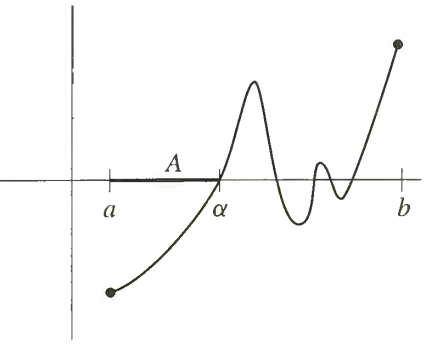
\includegraphics[scale=0.75]{IMV figure}
  \caption{}
\end{figure}

We now prove a lemma that will play a similar role to the proposition involved in the proof for intermediate value theorem.
\begin{lemma}
  If \(f\) is continuous at \(a\), then exists \(\delta\) such that \(f\) is bounded above (and below) in \((a-\delta,a+\delta)\). 
\end{lemma}
\begin{proof}
  We are given for all \(\epsilon\), exists \(\delta\) such that \(|x-a|<\delta\implies |f(x)-f(a)|<\epsilon\).

  Take \(\epsilon=1\), say. Then by triangle inequality,
  \[|x-a|<\delta\implies |f(x)|<|f(a)|+1\] 
  and so \(f\) is bounded above in \((a-\delta,a+\delta)\). Apply to \(-f\) for lower bound.
\end{proof}

The lemma can be extended easily to end points by considering \(\rointerval{a,a+\delta},\lointerval{b-\delta,b}\) and using definition of one-sided limits. Let's now prove the remaining two theorems.
\begin{theorem}[Boundedness Theorem]
  If \(f\) is continuous on \([a,b]\) then it is bounded (above and below) on \([a,b]\).
\end{theorem}
\begin{proof}
  Let \[A:=\{x\in[a,b]:f\text{ is bounded in }[a,x]\}\]
  Clearly \(A\neq\emptyset\) (\(a\in A\)) and is bounded (by \(b\)), so \(A\) has a supremum \(\alpha\in\R\). 
  
  We claim that \(\alpha = b\). Suppose that \(\alpha<b\). Then by lemma, exists \(\delta\) such that \(f\) is bounded in \((\alpha-\delta,\alpha+\delta)\). Pick some \(\alpha-\delta<x_0<\alpha\) and \(\alpha<x_1<\alpha+\delta\), we have \(f\) bounded in \([x_0,x_1]\). Also, \(x_0\in A\) so \(f\) bounded in \([a,x_0]\). But now \(f\) is bounded in \([a,x_1]\), i.e \(x_1\in A\) and \(x_1>\alpha\), a contradiction.

  We are not quite done yet: we have not considered the endpoints. However, we can prove them easily using the one-sided version of the lemma.

  We have \(\delta\) such that \(\{f(x):a\leq x <a+\delta\}\) is bounded, so \(\alpha\neq a\) (this is implicitly assumed in the argument above). Similarly, we have \(\{f(x):b-\delta<x\leq b\}\) is bounded for some \(\delta\). By above, there is \(b-\delta<x_0\leq b\) such that \(x_0\in A\). Hence, \(f\) is bounded on \([a,x_0]\) and \([x_0,b]\), thus on \([a,b]\) also.
\end{proof}
\begin{figure}[ht]
  \centering
  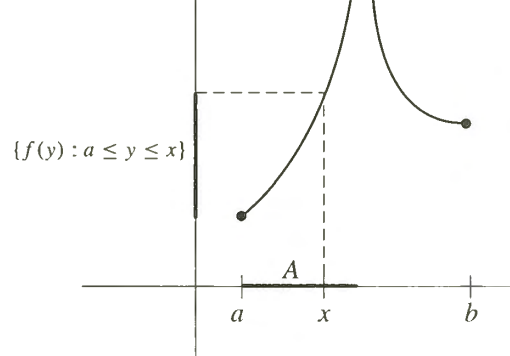
\includegraphics[scale=0.75]{Boundedness figure}
  \caption{}
\end{figure}

To prove the third theorem, we resort to a nice trick.
\begin{theorem}[Extreme Value Theorem]
  If \(f\) is continuous on \([a,b]\), then \(f\) must attain at least one maximum and one minimum, that is, there exist numbers \(c\) and \(d\) in \([a,b]\) such that:
  \[f(c)\leq f(x) \leq f(d), \forall x\in[a,b]\]
\end{theorem}
\begin{proof}
  We would just show the existence of \(d\) as the otherway is exactly the same.

  We know \(\{f(x):x\in[a,b]\}\) is bounded above and it is clearly not empty. We just need to show the supremum \(\alpha=f(x_0)\) for some \(x_0\in[a,b]\).
  
  Suppose this is not the case. Then the function
  \[g(x)=\frac{1}{\alpha-f(x)}\]
  is continuous in \([a,b]\) since the denominator is never \(0\). 

  Since \(\alpha=\sup(A)\), we know that for all \(\epsilon\), exists \(x\in[a,b]\) such that \(\alpha-f(x)<\epsilon\), i.e. \(g(x)>1/\epsilon\). But this means that \(g(x)\) is not bounded on \([a,b]\), a contradiction to boundedness theorem.
\end{proof}

Knowing these theorems, we can prove rigorously some results that you would have previously known, such as:
\begin{itemize}
  \item Every positive number has a square root.
  \item A monic (leading coefficient is 1) polynomial of degree \(n\) has at least one root if \(n\) is odd and a minimum/maximum value if \(n\) is even.
\end{itemize}

The converse of all three of these theorems are, however, not true. We can even find the extreme (pathological) counterexample where they are \emph{nowhere} continuous.
\begin{example}[Dirichlet function]
  The Dirichlet function given by
  \[D(x)=\begin{cases}
    1,& x\in\Q\\   
    0,& x\notin\Q
  \end{cases}\]
  is bounded by 1 and has maximum and minimum, but is nowhere continuous. Here is a proof of this.

  \begin{proof}
    Suppose \(D(x)\) is continuous at some point \(a\). Now fix \(\epsilon=\frac{1}{2}\). We have some \(\delta>0\) such that
    \[|x-a|<\delta\implies |D(x)-D(a)|<\epsilon\]

    Suppose \(a\notin\Q\) i.e. \(D(a)=0\). Then since \(\Q\) is dense in \(\R\) (see IUM), we can find \(x\in(a-\delta,a+\delta)\) such that \(x\in\Q\) i.e. \(D(x)=1\). 
    
    But now \(|D(x)-D(a)|=1>\frac{1}{2}\), a contradiction. The argument is exactly the same for \(x\in\Q\).

  \end{proof} 
\end{example}
\begin{problem}
  Prove that the function such that \(f(I)=\R\) for all open intervals \(I\) satisfies the intermediate value property but is nowhere conitnuous. Construct such a function.
\end{problem}
\begin{solution}
  Unseen 1 Q12,13
\end{solution}

\section{Derivatives}
\begin{definition}[Differentiability]
  A function \(f\) is differentiable at \(a\) if the limit
  \[\lim_{h\to 0}\frac{f(x+h)-f(x)}{h}\]
  exists. We call this limit the derivative of \(f\) at \(a\), denoted as \(f'(a)\) or \(\left.\diff{f}{x}\right\rvert_{x=a}\).

  A function is differentiable it is differentiable at \(x\) for all \(x\) in its domain.
\end{definition}
Of course, there is nothing stopping us taking higher-order derivatives \(f^(k)(x)\), where the function has been differentiated \(k\) times.


\begin{theorem}
  If a function \(f\) is differentiable, then \(f\) is continuous.
\end{theorem}
The converse is however not true.

\begin{example}[Weierstrass function]
  The Weierstrass function given by
  \[f(x)=\sum_{n=0}^{\infty}a^n\cos(b^n\pi x)\]
  where \(0<a<1, b\) a positive odd integer, and \(ab>1+\frac{3}{2}\pi\), is a pathological function that is continuous everywhere but differentiable nowhere. In fact, it is a fractal curve.

  One can show also that the sum of a differentiable function and the Weierstrass function is again continuous but nowhere differentiable. This means that there are at least as many such functions as differentiable functions. In fact, it has been proven that continuous functions are generically nowhere differentiable.
\end{example}

\begin{figure}[ht]
  \centering
  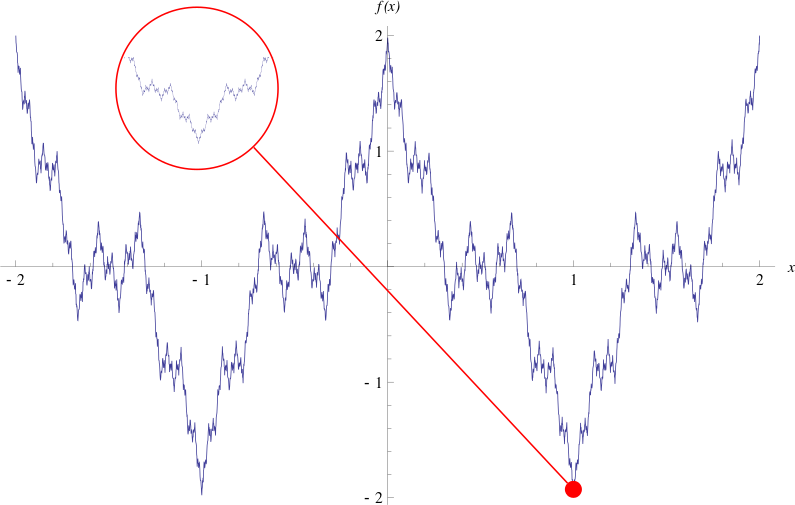
\includegraphics[scale=0.3]{Weierstrass function}
  \caption{Weierstrass function}
\end{figure}

\begin{theorem}
  If \(f,g\) are differentiable at \(a\), then \(f+g, f\circ g\) is also differentiable at \(a\).
\end{theorem}

\begin{definition}[Continuously differentiable]
  A function is continuously differentiable if its derivative is also continuous.
\end{definition}

To summarise, we have the following chain of strict inclusions for functions over a closed and bounded non-trivial interval of the real line:
\begin{center}
  Continuously differentiable \(\subset\) Lipschitz continuous \(\subset\) \(\alpha\)-Hölder continuous \(\subset\) uniformly continuous \(\subset\) continuous
\end{center}

% \begin{definition}[Open cover]
%   An open cover of \(A\subset\R\) is a set of open bounded intervals \(\{U_i:i\in I\}\) such that 
%   \[A\subseteq \bigcup_{i\in I}U_i\]
% \end{definition}

% \begin{theorem}[Heine-Borel theorem]
%   For a subset \(S\) or \(\R^n\), \(S\) is closed and bounded if and only if \(S\) is compact
% \end{theorem}

\begin{extension}{Cauchy functional equation}
  We are interested in functions \(f:\R\to\R\) such that for all \(x,y\in\R\),
  \[f(x+y)=f(x)+f(y)\]

  This is the Cauchy additive functional equation, and its solution is called additive function. One may notice straight away that \(f(x)=cx\) for some \(c\in\R\) is a linear solution. In fact, we can prove (see below) that under certain conditions, this is the only solution. However, non-linear pathological solutions do exist, and can serve as counterexample to advance questions.

  The following conditions preclude the pathological solutions:
  \begin{itemize}
    \item \(f\) is continuous at one point
    \item \(f\) is bounded on some interval
    \item \(f\) is monotonic on some interval
  \end{itemize}

  There are other types of Cauchy functional equation too:
  \begin{itemize}
    \item (exponential) \(f(x+y)=f(x)f(y)\)
    \item (logarithmic) \(f(xy)=f(x)+f(y)\)
    \item (multiplicative) \(f(xy)=f(x)f(y)\)
  \end{itemize}
\end{extension}

For derivatives of common functions and the product, quotient, and chain rule, see Calculus and Application. 

\section{Integral}
\end{document}